\documentclass[oneside]{tudelft-report}

\usepackage{verbatim}			% For comment-environment
\usepackage{enumitem}
\usepackage{parskip}
\usepackage{multicol}
\usepackage{multirow}
\usepackage[normalem]{ulem}
\usepackage{listings}
\usepackage{epstopdf}

\usepackage[section]{placeins}

\usepackage[nameinlink,capitalise]{cleveref}	% package for cref

\usepackage{subcaption} % For multiple subfigures in one figure
\usepackage{longtable}

%Todos
\usepackage{todonotes}
\newcommand{\todoi}{\todo[inline]}

% Colors and languages
\usepackage{color}


\definecolor{mygreen}{rgb}{0,0.6,0}
\definecolor{mygray}{rgb}{0.5,0.5,0.5}
\definecolor{mymauve}{rgb}{0.58,0,0.82}

\lstdefinestyle{MCRL2}{ %
  belowcaptionskip=1\baselineskip,
  breaklines=true,
  frame=single,
  xleftmargin=\parindent,
  showstringspaces=false,
  basicstyle=\footnotesize\ttfamily,
  keywordstyle=\bfseries\color{green!40!black},
  commentstyle=\itshape\color{purple!40!black},
  identifierstyle=\color{blue},
  stringstyle=\color{orange},
}

\lstset{
  backgroundcolor=\color{white},   % choose the background color; you must add \usepackage{color} or \usepackage{xcolor}
  basicstyle=\footnotesize,        % the size of the fonts that are used for the code
  breakatwhitespace=false,         % sets if automatic breaks should only happen at whitespace
  breaklines=true,                 % sets automatic line breaking
  captionpos=b,                    % sets the caption-position to bottom
  commentstyle=\color{mygreen},    % comment style
  keepspaces=true,                 % keeps spaces in text, useful for keeping indentation of code (possibly needs columns=flexible)
  keywordstyle=\color{blue},       % keyword style
  style=MCRL2,                 % the language of the code
  morekeywords={sum, true, false, init, allow, comm},    % if you want to add more keywords to the set
  morecomment=[l]{\%},
  numbers=none,                    % where to put the line-numbers; possible values are (none, left, right)
  numbersep=5pt,                   % how far the line-numbers are from the code
  numberstyle=\tiny\color{mygray}, % the style that is used for the line-numbers
  rulecolor=\color{black},         % if not set, the frame-color may be changed on line-breaks within not-black text (e.g. comments (green here))
  showspaces=false,                % show spaces everywhere adding particular underscores; it overrides 'showstringspaces'
  showstringspaces=false,          % underline spaces within strings only
  showtabs=false,                  % show tabs within strings adding particular underscores
  stepnumber=1,                    % the step between two line-numbers. If it's 1, each line will be numbered
  stringstyle=\color{mymauve},     % string literal style
  tabsize=2,                       % sets default tabsize to 2 spaces
  title=\lstname                   % show the filename of files included with \lstinputlisting; also try caption instead of title
}


%Commands for Parameter values
\newcommand{\on}{\textit{on}}
\newcommand{\off}{\textit{off}}
\newcommand{\error}{\textit{error}}
\newcommand{\up}{\textit{up}}
\newcommand{\down}{\textit{down}}
\newcommand{\stopped}{\textit{stopped}}
\newcommand{\stopi}{\textit{stop}}
\newcommand{\orange}{\textit{orange}}

% Titlepage
\begin{document}

%% Use Roman numerals for the page numbers of the title pages and table of
%% contents.
\frontmatter

\title[IN4387 Project: Group 6]{System Validation}
\author{W.F. Heida \and J.A. James \and E. Schoute \and  C. Tanaskoski}
\affiliation{Delft University of Technology}
\coverimage{cover/cover_blank.jpg}

\makecover

% Introduction
%\frontmatter
%\begin{center}
\Large \bf
Abstract

\todo[inline]{Write abstract}

\end{center}


\tableofcontents

% Lists
%\listoffigures
%\listoftables

%% Use Arabic numerals for the page numbers of the chapters.
\mainmatter

%Body
\chapter{Introduction}

	Following a car crash at the Ketelbrug, we started a design of a safety controller for bridges.
	Several safety concerns are in play, such as the one causing the previously mentioned accident, where the barriers were not closed before the bridge was opened.
	This was caused by an inexperienced operator using the emergency controls,
	which had become commonplace in the operation of that bridge due to problems with the standard controls~\cite{ProjectGuide}.
	
	The design of the bridge's safety controller will have to keep in mind both usability as well as safety.
	The safety of the traffic is the main focus of our safety controller,
	which will check if necessary precautions have been taken to prevent accidents.
	An example would be turning on stop lights before closing the barriers, allowing drivers to slow down in time.
	
	The bridge contains the following components: Pre-signs, Stop-signs, Barriers, Locking pins, Sensors, Brakes, and Motor.
	The safety controller will check the sensors of these components when operating the bridge, and when receiving user command, it will make appropriate decisions to guarantee safety. 
	In \cref{fig:situation} a situation sketch is shown of the system. 
	We assume that the pre-signs are placed a few hundred meters away from the bridge to give drivers an early warning that the bridge is not closed.
	
	\begin{figure}[!htbp]
		\begin{center}
		\includegraphics[width=0.6\textwidth]{images/Situation.png}
		\caption{The situation sketch of the system. ~\cite{ProjectGuide}}
		\label{fig:situation}
		\end{center}
	\end{figure}
	
	
	We will now provide the organization of this report. 
	In \cref{chap:requirements} the requirements for the safety controller will be discussed. 
	We will present the architecture of the safety controller in \cref{chap:systemarchitecture}. 
	In \cref{chap:interactions} the interactions between the controller and the other components of the system are described. 
	\cref{chap:tests} presents the transformation of the requirements presented earlier into more specific requirements containing the interactions. 
	This was done using mCRL2. 
	\cref{chap:model} provides information about the model design and all its components. 
	\cref{chap:verification} gives the verification results testing the model with the requirements.
	\cref{chap: conclusion} concludes this report.

\chapter{Model Requirements}\label{chap:requirements}
	As mentioned before, this safety controller should provide a safe environment in which bridge operators can control the bridge. 
	In order for us to ensure this, we began by specifying requirements to verify the safety and functionality of our design. 
	In this chapter we will first discuss the important model decisions that have been made, based on which our requirements were formulated. 
	Subsequently, we will provide the system global requirements. 
	  
	In our design we assume that there is an hardware mechanism present that ensures that the motor does not open/close the bridge beyond a maximum point. 
	This entails that if the user tries to open the bridge when it is already open, it will not be possible due to the hardware.
	Our safety controller is not responsible for resolving this error.
	
	There are two types of actions possible in the system. 
	The first type follows directly from a user command. 
	The second type of actions follow on the first type and are therefore indirectly related to a user command. 
	This means that the system is not allowed to perform actions that are completely initiated by itself.
	
	In the system it is allowed that one pre-sign and/or one stop sign is damaged. 
	Therefore such failures should not directly block the operation of the bridge. 
	If there are more failures the operation of the bridge should stop, because the system is then considered to be unsafe.


	\section{Functional Requirements}
		In order to ensure a proper operation of the safety controller for the bridge, we needed to define the specific behaviour of our system. 
		This was done by modelling the system behaviour with functional requirements.  
	 	
	 	
	 	 
		%First of all some functional requirements have to be defined to ensure a proper operation of the bridge.
		\begin{enumerate}
			% FR1
			\item The system should not contain any deadlocks.
			
			% FR2
			\item Cars should always have the possibility to safely pass the bridge.
			
			% FR3
			\item Boats should always have the possibility to safely pass the bridge.
		\end{enumerate}
	
	\section{Safety Requirements}
		To guarantee the safety of boats and cars, it was essential to define the specific system behaviour needed to make this possible. 
		We did this by providing the following safety requirements.
	
		\begin{enumerate}
			% SR1
			\item The stop signs should only be turned on when the pre signs are on.
			
			% SR2
			\item The barriers should only be closed when the stop-signs are on.
			
			% SR3
			\item The locking pins should only deactivate when the barriers are closed.
			
			% SR4
			\item The brakes should only be turned off when the locking pins are deactivated.
			
			% SR5
			\item The motor should only move upward when the brakes are disabled.
			
			% SR6
			\item The motor should only be stopped when the brakes is engaged.
			
			%SR7
				
			\item The locking pins should only activate when the motor has moved the bridge deck down.
		
			% SR8
			\item The barriers can only be opened when the locking pins are enabled.
			
			% SR9
			\item The stop signs should only be turned off when the barriers are opened.
			
			% SR10
			\item The pre-signs should only be turned off when the stop signs are off.
		\end{enumerate}

\chapter{System Architecture} \label{chap:systemarchitecture}
    In this chapter we discuss the architecture of the system's structure. The system architecture of the bridge contains four parallel components: the
	{\em safety controller}, {\em status controller}, the {\em hardware
	controller}, and the {\em sensors}. 
	They interact with each other and with the environment. 
	In this chapter we will discuss them in the same order respectively. 
	The	environment is defined by the user and the bridge's hardware as depicted in \cref{fig:arch}.
	The actions that were defined for the communication between the different components will be specified in \cref{chap:interactions}.
	
	\begin{figure}[htbp]
		\begin{center}
		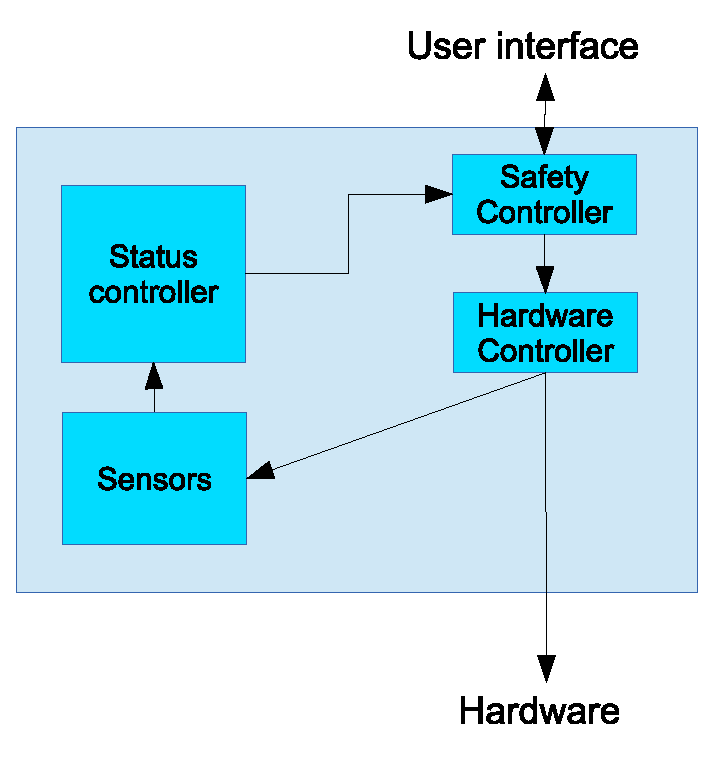
\includegraphics[width=0.6\textwidth]{./images/system-architecture.eps}
		\caption{The system architecture, components and their interactions}
		\label{fig:arch}
		\end{center}
	\end{figure}
	
	
	\section{Safety controller}
		The safety controller is embedded between the user interface and the hardware
		controller. 
		Its responsibility is to check whether the user's requests do not
		lead to an unsafe situation. 
		The checking of preconditions is performed based on the current state of the bridge.
		This information is retrieved from the status controller which is discussed in \cref{sec:arch:status}.
		
		If there is a threat to the safety it should not pass the request to the hardware controller and return an error message to the environment. 
		When the request is no threat to the safety of the system it should be forwarded to the hardware controller.
	
	
	
	\section{Status controller} \label{sec:arch:status}
		The status controller polls the sensors and aggregates information to determine the
		state of the bridge, whose main goal is to deal with inconsistent sensor data or a failure of a sensor. 
		When it is impossible to deduce correct information it should return an error to the user interface.
		It should also forward any other sensor errors that occur in the system like a error from the motor's sensor.
	
	
	
	\section{Hardware controller}
		All validated requests from the user are forwarded by the safety controller to the hardware controller.
		This component controls the hardware. 
		It can control the (pre-)signs, move the barriers, (dis)engage the locking pins and brakes, and control the engine. 
		The requests for opening and closing the bridge involve several actions of the system, which are issued by the safety controller in the right order. 
		The right order of these actions are specified in \cref{tbl:actionorder}
	
	\begin{table}[!htbp]
		\begin{center}
		\begin{tabular}{| l | l | l |}
			\hline
			Order & Opening the bridge 	& Closing the bridge	\\
			\hline
			1 & doPins(switch\_off) 	&	doMotor(motor\_down)	\\
			2 & doBrakes(switch\_off)	&	doBrakes(switch\_off)	\\
			3 & doMotor(motor\_up)		&	doMotor(motor\_stop)\\
			4 & doBrakes(switch\_on)	&	doBrakes(switch\_on)\\
			5 & doMotor(motor\_stop)	&	doPins(switch\_on)	\\
			\hline
		\end{tabular}
		\caption{The right order of actions for opening and closing the brigde.}
		\label{tbl:actionorder}
		\end{center}
	\end{table}

	\section{Sensors}
		The sensors component persists sensor information for four pre-signs, four stop-signs and the five other sensors. 
		The values returned by the sensors are not necessarily correct.
		It is the responsibility of the Status Controller to poll these sensors and handle any errors.


\chapter{Behaviour Interactions}	\label{chap:interactions}
    In this chapter we illustrate the interactions between the system components. We focus mainly on the global interactions.    
    In \cref{tbl:interactions} the external interactions between the components of the system are defined. 
	The interactions are grouped by communication pairs: user to safety controller, safety controller to user, safety controller to status controller, sensors to safety controller and the final pair safety controller to hardware controller.
	
	The interactions are based on the following assumptions.
	
	\begin{itemize}
	  \item Existence of a brake sensor such that the status of the brakes can be
	  determined. The idea is that the deck is not allowed to move if the brakes are
	  inoperable.
	  \item User does not need to control the motor, brakes and deck independently but
	  these interactions are grouped into 'userDeck(up) ' and 'userDeck(down)'.
	  \item Pre-signs are further away from the deck than the stop signs such that
	  the cars have time to slow down
	  \item Pre-signs stay on while the stop lights are on for the same reason as
	  above.
	  \item We assume all actions are instantaneous. This means that there is no
	  delay in our systems.
	\end{itemize}
	
	We decided that the user should not have direct control over the locking pins, brakes and motor for safety reasons. The only thing the user wants to do, is open or close the bridge. So there is no reason to let the user perform the right sequence of actions when you can also present two actions that take care of these sequences automatically, as illustrated in \cref{tbl:actionorder}. This will result in a system that can be used more easily by the bridge's operator.



	
\begin{center}
	\begin{longtable}{|l|p{8cm}|l|}
		\hline
		\textbf{Interaction name} & \textbf{Description} & \textbf{Parameters} \\ \hline
		\multicolumn{3}{c}{\textbf{User -> Safety Controller}} \\ \hline
		userPreSigns & Request the pre-signs to be turned on or off & Switch \\
		userStopSigns & Request the stop signs to be turned on or off & Switch \\
		userBarriers & Request the barriers to opened or closed & Switch \\
		userDeck & Request the deck to be opened or closed & Direction \\
		
		

		\hline 
		\multicolumn{3}{c}{\textbf{Safety Controller -> User}}\\ \hline
		prodError & Error occurred while executing request &   \\
		prodOK & OK message &   \\
	
		\hline
		\multicolumn{3}{c}{\textbf{Status -> Safety Controller}} \\ \hline
		checkStatusPreSigns & The status of the pre-signs & Status \\
		checkStatusStopSigns & The status of the stop-signs & Status \\
		checkStatusBarriers & The status of the barriers & Status \\
		checkStatusPins & The locking pins status & Status \\
		checkStatusBrakes & The brake status & Status \\
		checkStatusDeck & The bridge deck status & Status \\
		checkStatusMotor & The motor status & StatusMotor \\
		
		\hline
		\multicolumn{3}{c}{\textbf{Safety Controller -> Status}} \\ \hline
		startUpdateStatus & Request Status to poll the sensors for new information & \\
		endUpdateStatus & Synchronizes the Safety Controller to wait for polling to complete & \\
		
		\hline
		\multicolumn{3}{c}{\textbf{Hardware ->  Sensor}} \\ \hline                              
		changeSensorPreSigns & Change the sensor of the pre-signs & Status \\                   
		changeSensorStopSigns & Change the sensor of the stop-signs & Status \\                 
		changeSensorBarriers & Change the sensor of the barriers & Status \\                    
		changeSensorPins & Change the locking pins sensor & Status \\                           
		changeSensorBrakes & Change the brake sensor & Status \\                                
		changeSensorDeck & Change the bridge deck sensor & Status \\                            
		changeSensorMotor & Change the motor sensor & StatusMotor \\                            
		                                                                                        
		\hline
		\multicolumn{3}{c}{\textbf{Sensors -> Status}} \\ \hline 
		commSensorPreSignS$_{\{1,2,3,4\}}$ & Sensor status of the presigns. & Status \\
		commSensorStopSignS$_{\{1,2,3,4\}}$ & Sensor status of the stopsigns. & Status \\
		commSensorBarrierB$_{\{1,2\}}$ & Sensor status of the two barrier sensors. & Status \\
		commSensorPinP$_{\{1,2,\}}$ & Pin lock status sensors. & Status \\
		commSensorDeck & Bridgedeck status sensor. & Status \\
		commSensorMotor & Motor status sensor. & StatusMotor \\
		commSensorBrake & Bridge brake status sensor. & Status \\  

		\hline
		\multicolumn{3}{c}{\textbf{Safety Controller -> Hardware}} \\ \hline
		doPreSigns & All pre-signs are controlled with one signal. & Switch \\
		doStopSigns & All stop-signs are controlled with one signal. & Switch \\
		doBarriers & All barriers are controlled with one signal. & Switch \\
		doPins & All locking pins are controlled with one signal. On = engage, off = disengaged & Switch \\
		doBrakes & The bridge brakes are controlled. & Switch \\ 
		doMotor & The motor is set to specified setting. & SwitchMotor \\
		
		hwResponse & Hardware response. Occurs after sensors have been set & \\ \hline
		
		\caption{The interactions of the system.}
		\label{tbl:interactions}
	\end{longtable}	
\end{center}

In \cref{tbl:parameterTypes} the parameter types are defined that were used in \cref{tbl:interactions}.



\begin{table}[htbp]	
	\centering
	\begin{tabular}{|l|l|}
		\hline
    	\textbf{Parameter type} & \textbf{Set of values} \\ \hline
    	Status				& on, off, error			\\
    % % %	statusDirection		& up, down, error			\\
    	StatusMotor			& status\_up, status\_down, status\_stopped, status\_error	\\
    	Switch				& switch\_on, switch\_off					\\
    	Direction			& up, down					\\
    	SwitchMotor			& motor\_up, motor\_down, motor\_stop			\\ \hline
	\end{tabular}
	\caption{The table of parameter types.}
	\label{tbl:parameterTypes}
\end{table}

\begin{comment}
errorLightsOn & The	requested action can not be performed since the lights are on &
		\\
		errorLightsOff & The requested action can not be performed since the lights
		are off &
		\\
		errorBarriersOpen & The requested action can not be performed since the
		barriers are open & 
		\\
		errorBarriersClosed & The requested action can not be performed since the
		barriers are closed &
		\\
		errorDeckOpen & The requested action can not be performed since the deck is
		open & 
		\\
		errorDeckClosed & The requested action can not be performed since the desk is closed &
		\\
\end{comment}
\chapter{Specified Requirements} \label{chap:tests}



In this chapter we will look more closely at the requirements specified in \cref{chap:requirements}. 
We will translate the requirements from full natural language to natural language containing the interactions defined in \cref{chap:interactions}.
This will make the requirements more specific and will make the translation to $\mu$-Calculus easier.
The following numeration follows that of the general requirements.

Tests add to each other transitively,
which means that if one test checks the safety requirements of object A and B,
and another tests the requirements for B and C,
then it is assumed that A and C together function correctly if they only have interactions through B.


\section{Functional Requirements}

\begin{enumerate}
	% FR1
	\item For all traces in the system, the system should end in a state in which a step is possible.
	\lstinputlisting[firstline=4, lastline=4, caption={FR1.mcf}]{source/FR1.mcf}


	% FR2
	\item For all states there should be a path that contains the action doPreSigns(switch\_off).
	\lstinputlisting[firstline=4, lastline=4, caption={FR2.mcf}]{source/FR2.mcf}	

	
	% FR3
	\item For all states there should be a path that contains the action doMotor(motor\_up).
	\lstinputlisting[firstline=4, lastline=4, caption={FR3.mcf}]{source/FR3.mcf}


\end{enumerate}

\section{Safety Requirements}
\begin{enumerate}


	% SR1	
	\item doPreSigns(switch\_off) may never be followed by doStopSigns(switch\_on) unless doPreSigns(switch\_on) and checkStatusPreSigns(on) happened intermediately.
	\lstinputlisting[firstline=4, lastline=6, caption={SR1a.mcf}]{source/SR1a.mcf}
	
	
	% SR2
	\item doStopSigns(switch\_off) may never be followed by doBarriers(switch\_on) unless doStopSigns(switch\_on) and checkStatusStopSigns(on) happened intermediately.
	\lstinputlisting[firstline=4, lastline=6, caption={SR2a.mcf}]{source/SR2a.mcf}
	
	
	% SR3
	\item doBarriers(switch\_off) may never be followed by doPins(switch\_off) unless doBarriers(switch\_on) and checkStatusBarriers(on) happened intermediately. 
	\lstinputlisting[firstline=4, lastline=6, caption={SR3a.mcf}]{source/SR3a.mcf}
	
	
	% SR4	
	\item doPins(switch\_on) may never be followed by doBrakes(switch\_off) unless doPins(switch\_off) and checkStatusPins(off) happened intermediately. 
	\lstinputlisting[firstline=4, lastline=6, caption={SR4a.mcf}]{source/SR4a.mcf}
	
	% SR5
	\item doBrakes(switch\_on) may never be followed by doMotor(switch\_up) unless doBrakes(switch\_off) and checkStatusBrakes(off) happened intermediately. 
	\lstinputlisting[firstline=4, lastline=6, caption={SR5a.mcf}]{source/SR5a.mcf}
	
	
	% SR6
	\item doBrakes(switch\_off) may never be followed by doMotor(motor\_stop) unless doBrakes(switch\_on) and checkStatusBrakes(on) happened intermediately. 
	\lstinputlisting[firstline=4, lastline=6, caption={SR6a.mcf}]{source/SR6a.mcf}
		

	% SR7	
	\item doMotor(motor\_up) may never be followed by doPins(switch\_on) unless doMotor(motor\_down) and checkStatusMotor(status\_down) happened intermediately. 
	\lstinputlisting[firstline=4, lastline=6, caption={SR7a.mcf}]{source/SR7a.mcf}
	
	
	% SR8
	\item doPins(switch\_off) may never be followed by doBarriers(switch\_off) unless doPins(switch\_on) and checkStatusPins(on) happened intermediately. 
	\lstinputlisting[firstline=4, lastline=6, caption={SR8a.mcf}]{source/SR8a.mcf}
	
	
	% SR9
	\item doBarriers(switch\_on) may never be followed by doStopSigns(switch\_off) unless doBarriers(switch\_off) and checkStatusBarriers(off) happened intermediately.
	\lstinputlisting[firstline=4, lastline=6, caption={SR9a.mcf}]{source/SR9a.mcf}
		
	
	%SR 10
	\item doStopSigns(switch\_on) may never be followed by doPreSigns(switch\_off) unless doStopSigns(switch\_off) and checkStatusStopSigns(off) happened intermediately. 
	\lstinputlisting[firstline=4, lastline=6, caption={SR10a.mcf}]{source/SR10a.mcf}
	
	
\end{enumerate}


\section{Additional tests}

	The $\mu$-calculus properties for the requirements that were presented so far, give equations that test whether certain paths are tested are always reachable or that certain sequences of actions can never happen.
	To ensure that the safety requirements do not hold vacuously we also performed some additional tests.
	
	
	\subsection{Trivial paths}
	
	These tests include several properties that verify that the actions  used in the requirements can be reached in the system.
	We call these properties the trivial paths.
	If these actions cannot be reached or do not exist, it is clear that the requirements will hold for the system, but do not have any meaning.
	We have performed the verification of the trivial path for five requirements.
	In \cref{ver_tr_SR1} an example of one of the properties is given that tests if the trivial path to the action doStopSigns(switch\_off) exists.
	Likewise, we have formulated properties for all other actions that were used in the safety requirements.
	
	\begin{lstlisting}[caption=SR1 trivial path example ,label=ver_tr_SR1] 
	<true* . doStopSigns(switch_off) >true 
	\end{lstlisting}


	\subsection{Existential tests}
	
    The properties for the trivial paths do not give a full proof that paths exist between the actions that form the safety requirements. 
    They only test if the possible actions adhere to those specified in the safety requirements. 
    Therefore we also added existential tests. 
    These properties test if a path exists between the two most important actions in the safety requirements. 
    These properties can be found below.
    We do not need to eliminate a \texttt{doX} action from the intermediate steps where $X$ is a component,
    because a \texttt{checkStatus} action is always performed before any \texttt{doX} action.
    This means that through the sensors we know that the current state of the component has not changed from the expected state.
    
    \begin{enumerate}
    
    
    	% SR1	
    	\item doPreSigns(switch\_on) can be followed by doStopSigns(switch\_on) without checkStatusPreSigns(off) or checkStatusPreSigns(error) happening intermediately.
    	\lstinputlisting[firstline=4, lastline=6, caption={SR1b.mcf}]{source/SR1b.mcf}
    	
    	
    	% SR2
    	\item doStopSigns(switch\_on) can be followed by doBarriers(switch\_on) without checkStatusStopSigns(off) or checkStatusStopSigns(error) happening intermediately.
    	\lstinputlisting[firstline=4, lastline=6, caption={SR2b.mcf}]{source/SR2b.mcf}
    	
    	
    	% SR3
    	\item doBarriers(switch\_on) can be followed by doPins(switch\_off) without checkStatusBarriers(off) or checkStatusBarriers(error) happening intermediately.
    	\lstinputlisting[firstline=4, lastline=6, caption={SR3b.mcf}]{source/SR3b.mcf}
    	
    	
    	% SR4	
    	\item doPins(switch\_off) can be followed by doBrakes(switch\_off) without checkStatusPins(off) or checkStatusPins(error) happening intermediately. 
    	\lstinputlisting[firstline=4, lastline=6, caption={SR4b.mcf}]{source/SR4b.mcf}
    	
    	% SR5
    	\item doBrakes(switch\_off) can be followed by doMotor(motor\_up) without checkStatusBrakes(on) or checkStatusBrakes(error) happening intermediately.
    	\lstinputlisting[firstline=4, lastline=6, caption={SR5b.mcf}]{source/SR5b.mcf}
    	
    	
    	% SR6
    	\item doBrakes(switch\_on) can be followed by doMotor(motor\_stop) without checkStatusBrakes(off) or checkStatusBrakes(error) happening intermediately.
    	\lstinputlisting[firstline=4, lastline=6, caption={SR6b.mcf}]{source/SR6b.mcf}
    		
    
    	% SR7	
    	\item doMotor(motor\_down) can be followed by doPins(switch\_on) without checkStatusMotor(status\_up), checkStatusMotor(status\_error) or checkStatusMotor(status\_stopped) happening intermediately. 
    	\lstinputlisting[firstline=4, lastline=6, caption={SR7b.mcf}]{source/SR7b.mcf}
    	
    	
    	% SR8
    	\item doPins(switch\_on) can be followed by doBarriers(switch\_off) without checkStatusPins(on) or checkStatusPins(error) happening intermediately. 
    	\lstinputlisting[firstline=4, lastline=6, caption={SR8b.mcf}]{source/SR8b.mcf}
    	
    	
    	% SR9
    	\item doBarriers(switch\_off) can be followed by doStopSigns(switch\_off) without checkStatusBarriers(on) or checkStatusBarriers(error) happening intermediately.
    	\lstinputlisting[firstline=4, lastline=6, caption={SR9b.mcf}]{source/SR9b.mcf}
    		
    	
    	%SR 10
    	\item doStopSigns(switch\_off) can be followed by doPreSigns(switch\_off) without checkStatusStopSigns(on) or checkStatusStopSigns(error) happening intermediately. 
    	\lstinputlisting[firstline=4, lastline=6, caption={SR10b.mcf}]{source/SR10b.mcf}
    	
    	
    \end{enumerate}


	\section{Sensors Testing}
	
	We have also tested the sensors in order to ensure that an error status is received when one or more sensors are not working or the component is broken.  
	
	We built a significant number of sensors into our system, so this would require a large amount of properties to fully test them. 
	Because we didn't have time to do that, we have chosen to tests the pre-sign sensors only.
	There are four pre-sign sensors which need to be aggregated into one status.
	Also one pre-sign or pre-sign sensor may fail without the operation of the bridge being blocked.
	If the tests for the pre-sign sensors succeed we can assume that the other sensors have been implemented in a correct fashion as well.
	
	One important thing to note is that all sensors for one particular component are the same, so we can assume that the sensors are symmetrical.
	This reduces the number of cases with different sensor values that have to be tested by a significant amount.
	In \cref{lst:Sensor_1a} until \cref{lst:Sensor_3a} the 3 properties that were used to test the sensor are given.
	
	\begin{enumerate}
		\item There exists no path where for all combinations that include 2 or more sensor values that are error the status will be on or off. 
		\lstinputlisting[firstline=4, lastline=15, caption={Sensor\_PreSign1a}, label={lst:Sensor_1a}]{source/Sensor_PreSign1a.mcf}
			
		\item There exists no path where for all combinations that include 3 or more sensor values that are on the status will be not be error or off.
		\lstinputlisting[firstline=4, lastline=15, caption={Sensor\_PreSign2a}, label={lst:Sensor_2a}]{source/Sensor_PreSign2a.mcf}
		
		\item There exists no path where for all combinations that include 3 or more sensor values that are off the status will be not be error or on.
		\lstinputlisting[firstline=4, lastline=15, caption={Sensor\_PreSign3a}, label={lst:Sensor_3a}]{source/Sensor_PreSign3a.mcf}
	\end{enumerate}
	
	To make sure that these properties do not hold vacuously, we also implemented 3 conresponding existential tests.
	These existential tests are given in \cref{lst:Sensor_1b} until \cref{lst:Sensor_3b}.
	
	\begin{enumerate}
		\item There exists a path where for all combinations that include 2 or more sensor values that are error the status will be error. 
		\lstinputlisting[firstline=4, lastline=15, caption={Sensor\_PreSign1a.mcf}, label={lst:Sensor_1b}]{source/Sensor_PreSign1b.mcf}
			
		\item There exists a path where for all combinations that include 3 or more sensor values that are on the status will be on. 
		\lstinputlisting[firstline=4, lastline=15, caption={Sensor\_PreSign2a.mcf}, label={lst:Sensor_2b}]{source/Sensor_PreSign2b.mcf}
		
		\item There exists a path where for all combinations that include 3 or more sensor values that are off the status will be off. 
		\lstinputlisting[firstline=4, lastline=15, caption={Sensor\_PreSign3a.mcf}, label={lst:Sensor_3b}]{source/Sensor_PreSign3b.mcf}
	\end{enumerate}
	
	
	In \cref{chap:verification} the results of the verification of all the properties that were given before will be presented.
\chapter{Model Design}	\label{chap:model}
	In earlier chapters we have identified the processes of the Status, Sensors, Safety and Hardware Controller.
	We have kept these processes separated according to the identified processes.
	The list of processes is as follows:
	\begin{description}
		\item[SafetyController] the controller responsible for security:
			\begin{description}
				\item[SafetyPreSigns] handles the safety aspect of the pre-signs.
				\item[SafetyStopSigns] idem for the stop signs.
				\item[SafetyBarriers] idem for the barriers.
				\item[SafetyDeck] idem for the deck.
					\begin{description}
						\item[SafetyDeck\_Pins] component of the deck safety controller that handles the pins.
						\item[SafetyDeck\_Brakes] idem for the brakes.
						\item[SafetyDeck\_Motor] idem for the motor.
					\end{description}
			\end{description}
		\item[HardwareController] the controller responsible for modelling the hardware layer.
		\item[StatusController] the controller responsible for storing the sensor status of bridge components.
		\item[Sensors] models the sensor behaviour. 
	\end{description}



	The resulting LTS model has $170$ levels, $247,940$ states and $358,268$ transitions.
	The number of states exploded when we added code for processing the sensor handling.
	In particular the code given in~\cref{list:sensorpolling} causes a large number of states,
	because of the many types of values the variables can assume: $3^{12}\cdot4 > 2\cdot 10^6$.
	Additionally, a graphical representation of the state space is given in~\cref{fig:statespace}

	\lstinputlisting[style=MCRL2, caption={The polling of sensor state in the StatusController}, label={list:sensorpolling}]{source/sensorpolling.mcrl2}

	\begin{figure}[h]
		\centering
		\includegraphics[height=0.4\textheight]{images/state_model.png}
		\caption{3D State space model of the entire system}
		\label{fig:statespace}
	\end{figure}

	\section{Safety Controller}
		The safety controller has several sub-processes handling the behaviour of each possible user input.		
		Because we assumed that the user has only inputs for pre-signs,
		stop-signs, barriers and the bridge deck there are only 4 of these sub-processes.
 
		Each sub-process first checks if the relevant component does not have the \texttt{error} sensor state.
		Then, depending on the user input, the required state is checked,
		e.g. for turning the stop signs on the pre-signs have to be on.
		But for turning the stop signs off the barriers have to be off instead.
		Then the Hardware Controller is requested to execute the user request,
 if the state is as expected.
 	 A Produce OK (\texttt{ProdOK}) is executed if everything went as expected,
 	 Produce Error (\texttt{ProdError}) if a requirement was not met.

 	 The deck safety controller was split into several sub-processes,
 	 because opening the bridge deck is a complex interplay of three bridge components:
 	 the locking pins, the brakes and the motor.
 	 To save space we introduced a \texttt{Direction} type as additional argument,
 	 which allows us to reuse the sub-process in both up and downward operation of the bridge deck.
 	 While the number of branches can be large at times (see \texttt{SafetyDeck\_Motor}),
 	 the behaviour is simple and very similar to a finite state machine. 

	\section{Hardware Controller}
		The goal of the hardware controller is modelling the hardware behaviour.
		All this does in our system is setting the sensor status of the requested component to the correct type.
		This process could be extended to perform hardware routines.

	\section{Status Controller}
		The status controller offers both functionality to poll sensor data and aggregate the results,
		and to read the aggregated data that is saved in its state.
		We use a polling method for reading the sensors,
		because analysing this is easier than an asynchronous process that can update the state at any time.

		The polling of all sensors is performed in one block of code after a \texttt{startUpdateStatus} request.
		Even though this is not very efficient in the number of the states,
		the code remains well readable this way.
		The status of the signs are stored inside \texttt{Bag} objects,
		which we can later use to calculate the number of \texttt{on}, \texttt{off} and \texttt{error} states of the signs.
		After polling the sensors, this data is saved in the state of the status controller for later reading.

		The reading can be done with a \texttt{checkStatusX} request,
		where $X$ is a component.
		This is straightforward reading from the current state of the status controller,
		except for the signs.
		The signs have as additional requirement that if just one sign has an error sensor state,
		that the bridge can still remain operational.
		To this end we created the Bags at the sensor polling phase,
		because now it is easy to count the number of occurrences of states in and conclude the appropriate aggregated sign state.
		
		The initial values of the status of the components are given in \cref{tbl:statusinit}.
		
		\begin{table}[!htbp]
			\begin{center}
			\begin{tabular}{l l}
				\hline
				Status				& Value	\\
				\hline
				statusPreSignBag	&	{off:4, on: 0, error:0}		\\
				statusStopSignBag	&	{off:4, on:0, error:0}		\\
				statusBarriers		&	off		\\
				statusBrakes		&	on		\\
				statusPins			&	on		\\
				statusDeck			&	off		\\
				statusMotor			&	status\_stopped	\\
				\hline
			\end{tabular}
			\caption{The initial values of the status of the components}
			\label{tbl:statusinit}
			\end{center}
		\end{table}

	\section{Sensors} \label{sec:sensors}
		The sensors are a simple sub-process that keep track of the current sensor state of the components.
		When the hardware changes it notifies the sensors so that the state may be updated.
		Requests to the sensors can be achieved with \texttt{commSensorX} action. 
		To model possible defects in the system, there is a possibility to return an \texttt{error} state for each communication.
		This way it is possible for a sensor to return an error state independent of the hardware controller.
		The sensor are initialized with the values as listed in \cref{tbl:sensorinit}.
		
		\begin{table}[!htbp]
			\begin{center}
			\begin{tabular}{l l}
				\hline
				Sensor	& Value	\\
				\hline
				sensorPreSigns	&	off	\\
				sensorStopSigns	&	off	\\
				sensorBarriers	&	off	\\
				sensorPins		&	on	\\
				sensorBrakes	&	on	\\
				sensorDeck		&	off	\\
				sensorMotor		&	status\_stopped\\
				\hline
			\end{tabular}
			\caption{The initial value of the sensors}
			\label{tbl:sensorinit}
			\end{center}
		\end{table}
	

	\section{Initialization}
		In \cref{list:initialization} the initialization of the processes in our model is given. Also all actions that are allowed and the corresponding communicating actions are declared here. Finally the parallel processes are initialized with the correct initial values for the sensors and the status of all the components.
		The various controllers are run in parallel and synchronized using the communication actions.
		The initial state of the model is set in both the \texttt{StatusController} as well as the \texttt{Sensors}.
		For the \texttt{StatusControler} it is assumed that:
		\begin{enumerate}
			\item all the signs are off
			\item the barriers are open (off)
			\item the brakes are on
			\item the pins are engaged (on)
			\item the deck is down (off)
			\item the motor is off (status\_stopped)
		\end{enumerate}
		The same holds for the initial state of the \texttt{Sensors}.
		
		\lstinputlisting[style=MCRL2, caption={The initialization of the mCRL2 model.}, label={list:initialization}]{source/initialization.mcrl2}
\chapter{Verification Results}	\label{chap:verification}
	In order to test whether the model satisfies the requirements specified in \cref{chap:requirements} the accompanying $\mu$-calculus formulas in \cref{chap:tests} have to be tested.
	In this chapter a detailed description of how the verification process was carried out is given.
	
	The verification was done using the mCRL2 toolset~\cite{mcrl2website}. 
	Tools such as \texttt{mcrl22lps} , \texttt{lps2pbes} and \texttt{pbes2bool} were used in this process.
	The version of the mCRL2 toolset used is \texttt{201310.0 (Release)}.
	
	The \texttt{mcrl22lps} tool takes the process specification from our model as input and converts it to a Linear Process System, see \cref{mcrl22lps}. 
	
	\begin{lstlisting}[caption=Transformation of mCRL2 model to LPS description, label=mcrl22lps ]
	mcrl22lps model.mcrl2 model.lps
	\end{lstlisting}
	
	With the model in {\em lps-format} the tests can be run with command
	\cref{ver_cmd} where {\em <requirement>} is the name of	the requirement at hand, for example {\em SR3}.
	The tool \texttt{lps2pbes} was used to create a parameterised boolean equation system (PBES) from the LPS description of our model and the requirement at hand.
	The result is piped to \texttt{pbes2bool} to retrieve
	the boolean value which shows whether the test passes or not.
	 
	\begin{lstlisting}[caption=Requirement testing ,label=ver_cmd] 
	lps2pbes model.lps -f <requirement>.mcf | pbes2bool
	\end{lstlisting}

	There are many tests to run and  each test takes a minute or two to compute. To speed up the process the tests were run in parallel using GNU Parallel\cite{Tange2011a}. The \cref{ver_cmd_parallel} shows
	the command used to speed up the verification with at least a factor four.
	\begin{lstlisting}[caption=Parallelization of verification command, label=ver_cmd_parallel]
	parallel -k --tag 'lps2pbes model.lps -f {} | pbes2bool' ::: *.mcf
	\end{lstlisting}
	
	\cref{tbl:verificationResults} depicts the results of running all 13
	tests listed in \cref{chap:tests} .
	The results show that the model passed all the functional and safety requirements.
	This indicates that the model can be considered safe.
		
	\begin{table}[!htbp]
		\begin{center}
		\begin{tabular}{l | r r}
			Requirement type & \# passed & \# failed \\ \hline
			Functional & 3 & 0 \\
			Safety & 10 & 0	\\
		\end{tabular}
		\caption{Model verification results}
		\label{tbl:verificationResults}
		\end{center}
	\end{table}

	
	\cref{tbl:trivialResults} depicts the results of running all properties for the trivial paths and the existential tests. 
	The results show that all trivial paths exist for the first five requirements.
	It can also be seen that all existential tests pass, so all paths that should exist according to our safety requirements do actually exist.
	Based on these results we can conclude that the safety requirements do not hold vacuously.
		
	\begin{table}[!htbp]
		\begin{center}
		\begin{tabular}{l | r r}
			Property type & \# passed & \# failed \\ \hline
			Trivial paths & 23 & 0	\\
			Existential tests	&	10	&	0	\\
		\end{tabular}
		\caption{The verification results of the trivial paths and existential tests}
		\label{tbl:trivialResults}
		\end{center}
	\end{table}
	
	\cref{tbl:sensorResults} depicts the results of running all properties for the sensors.
	The results show that the implementation of the sensors passes all requirements
	
	\begin{table}[!htbp]
		\begin{center}
		\begin{tabular}{l | r r}
		Property type	& \# passed & \# failed \\	\hline
		Sensor			& 3	& 0 \\
		Existential tests & 3 & 0 \\
		\end{tabular}
		\caption{The verification results for the sensors}
		\label{tbl:sensorResults}
		\end{center}
	\end{table}
	   
   

\chapter{Discussion \& Conclusions}	\label{chap: conclusion}
	In this project we aimed to design a safety controller which takes commands from the bridge operator 
	and presents them to the hardware, while taking in mind security of bridge operation.
	It was essential that this happens in a safe way, to prevent future accidents from happening.
	
	In order to build our system, we made some assumptions to simplify the design of the safety controller.
	One important assumption was that the user does not need to control the motor,
	brakes and deck independently. % I'm not sure if this is the 'most important one'
	This is done by a grouping interactions into one single command for the user.
	We designed a model which consists of four components: safety controller, hardware controller, status controller, and sensors.  
	
	We verified the safety of the model with functional and safely requirement using the MCRL2 tools.
	The model passed all tests and it is therefore considered to meet the requirements and is considered safe.
	Even though the model passed all test, it should be clear that this does not mean that this design can be used in the real world.
	Before this can happen, it still requires more strict safety requirements to ensure that the system does not fail.
	However, this model still demonstrates the beginnings of a bridge controller that adheres to safety requirements. 
 

% Appendix
%\appendix


% Bibliography
%\begin{thebibliography}{9}
%\bibliographystyle{IEEEtran} % Doesn't work with tudelft-report.bst
\bibliography{IEEEabrv,literature}
%\end{thebibliography}

\end{document}
